\documentclass{article}
\usepackage{graphicx} % Required for inserting images
\usepackage{natbib}
\usepackage{amsmath}
%\usepackage{comment}
\usepackage{url} 
%\usepackage[hidelinks]{hyperref}
%\usepackage[T1]{fontenc}
%\usepackage{mathpazo,euler}
%\usepackage[scaled=0.9]{DejaVuSans}
%\usepackage[utf8]{inputenc}
\usepackage{listings}
\usepackage{tabularx}
%\usepackage{amsfonts}
%\usepackage{booktabs}
%\usepackage{siunitx}
\usepackage{geometry}
%\usepackage[font=tiny,labelfont=bf]{caption}
\usepackage{float} % At the beginning of your document
\geometry{margin=1.5in}
%\lstset{basicstyle=\ttfamily}
%\documentclass[11pt]{article}
%\setlength{\parskip}{1em} % 1em is an example value; adjust as needed
\bibliographystyle{abbrvnat}
\setcitestyle{authoryear,open={(},close={)}} % Citation-related commands

%\title{First Year Paper}
\title{The implications of genetic architecture on rapid evolutionary outcomes} % Add your subtitle here
% title ideas
% Genetic architecture implication on rapid evolutionary dynamics & detectability of causal loci after a rapid evolution event 



%\subtitle(Advisor: Moisés Expósito Alonso)
\author{Tatiana Bellagio \\ Advisor: Moisés Expósito Alonso}
\date{November 2023}

\let\oldparagraph\paragraph
\renewcommand{\paragraph}[1]{\oldparagraph{#1}\mbox{}\\}

\begin{document}

\maketitle

\begin{abstract}
In the face of anthropogenic climate and land use crises, environments are changing faster than ever and species must adapt to keep up and avoid extinction. While this has motivated much theoretical and simulation-based research to study the role of genetic architecture in rapid environmental adaptation, these studies are rarely parameterized with realistic setups let alone validated through feasible experiments. Here, I use population genetic simulations varying genetic architecture parameters, from monogenic to polygenic, from low heritable to high heritable traits, coded by low to high-frequency alleles, in experimental setups that closely match an experimental evolution design with \textit{Arabidopsis thaliana}. This includes realistic population sizes, survival and fecundity distributions, partial selfing, strengths of selection through simulations with real whole-genome variant data. I then investigate the effect of such parameters and the outcome of population adaptation or extinction. My results indicate that traits with higher polygenicity significantly enhance survival probabilities in rapidly changing environments, while the influence of heritability, contrary to common intuition, is context dependent with positive or negative influence depending on genetic architecture complexity.
\end{abstract}
\newpage % Starts a new page after the table of contents
\tableofcontents
\newpage % Starts a new page after the table of contents

\section{Introduction}
\subsection{Shift, Adapt or Perish}
When species face environmental changes that displace them from their ecological niche, there are only three possible outcomes: shift their geographical distribution to track suitable environments, adapt to the newly imposed conditions, or face local to global extinction. Adaptation is the process by which a population becomes better suited to the new environment through natural selection acting over the population's standing and de novo genetic variation. In the face of rapid anthropogenic environmental changes \citep{IPCC2023}, adaptation through evolution must also be rapid to ensure populations' persistence and avoid extinction. Thus, specifically understanding rapid eco-evolutionary dynamics and outcomes has become of utmost importance \citep{Waldvogel2020-dh, Palumbi2002-li, Stockwell2003-da}. 

\subsection{What is rapid evolution?}
Evolution has been historically thought of as a slow and gradual process occurring over extensive timescales, often spanning thousands to millions of years. However, genetically based rapid phenotypic changes have been shown to be pervasive in nature, such as the famous peppered moth \citep{Cook2013-bs}, insecticide resistance in \textit{Drosophila} \citep{Daborn2002-is}, beak size in Darwin’s finches \citep{Grant2008-uc}, \textit{Brassica rapa} flowering time in response to climate fluctuations \citep{Franks2007-ys}, and the evolved resistance to agricultural products in more than 200 plant species \citep{Heap2020}. 

Rapid evolution can be defined based on the short number of generations in which a genetic change occurs, but also as the convergence of ecological and evolutionary times \citep{Hairston2005-qo}. This highlights the importance of rapid evolution as one of the more applied domains within evolutionary biology. Coupled with advances in genome sequencing technology that have led to an increase in the genomic data on non-model organisms, the understanding of eco-evolutionary dynamics has the potential to address urgent conservation issues. Understanding and predicting the pace and direction of evolutionary changes can inform conservation strategies and management practices. \citep{Bay2017-uu, Coulson2017-yh, Forester2022-yl}.

As highlighted in \citep{Yamamichi2022-yj} short-term eco-evolutionary dynamics, despite their inherent interdisciplinary nature, have been mostly studied solely from an ecological perspective and tend to focus on adaptation at the phenotypic level without considering the genetic part of the evolutionary process. More studies are needed in the evolutionary aspect of rapid adaptation to understand intertwined processes and to make more accurate predictions. \citep{Rudman2022-uc}

\subsection{Trait architecture and its potential impact in adaptation}
Discussions concerning how and where adaptive loci are distributed across the genome have come a long way. Since Darwin \citeyearpar{Darwin1859-yh} and Huxley \citeyearpar{Huxley1860} there have been debates about whether the nature of adaptation is characterized by incremental, subtle variations in many loci or by abrupt changes on only a few of them. These are foundational unsolved questions in evolutionary biology, with compelling evidence showing that both cases can be true and that there is considerable heterogeneity in architectures among adaptive traits \citep{Orr1992-xj, Orr1998-pr}, not to mention the complexities not discussed here, including the effect of structural variation, epistasis, pleiotropy, and ploidy. 

The implications of genetic architecture on population dynamics have been widely documented. For example, genetic architecture acting as a buffer for adaptive alleles through dominance \citep{Yamamichi2017-uj}, or the implication of the number of loci affecting reproductive incompatibility and determining speciation \citep{Orr1996-eq}. Many more are listed in \citep{Bertram2019-sg}. Delving deeper into a more narrow definition of genetic architecture--defined as the number, frequency, distribution of effects and penetrance of causal loci-- two qualitatively different waves of research can be described. The first, rooted in traditional population genetics, focuses on selective sweeps where adaptation depends only on one or a few high-effect adaptive loci \citep{Hermisson2005-ii,Barrett2008-tj}. The second, emerging from quantitative genetics and strengthened by the advent of sequencing technologies and statistical methodologies, focuses on the evolutionary dynamics of polygenic traits coded by many low-effect loci \citep{John2020-xc, Jain2017-mb, Barghi2020-aa, Hayward2021-ji, Stetter2018-st, Thornton2019-ww, Hollinger2019-lb}. 

\subsection{Gap in understanding the genetic architecture of rapid adaptation}
However, often these studies focus on the impact of genome architecture in adaptation in general, spanning long periods and extending over hundreds or thousands of generations and relying on a tremendous amount of \textit{de novo} mutations, rather than studying their impacts in short, rapid adaptation. As shown by \citep{Orr2008-jl}, adaptation to big environmental challenges over short periods can be difficult when relying on new mutations, and populations will often decline to extinction. Instead, rapid adaptation is likely to proceed through standing genetic variation \citep{Barrett2008-tj}. The implication of different trait genetic architectures from standing genetic variation on the outcomes of rapid evolution has been limited to a handful of studies \citep{Gomulkiewicz2010-wr, Kardos2021-jd}, showing conflicting results, and often conducted in highly abstract simulations and theoretical parameter spaces.

Since the relationship between different genetic architectures and the outcomes of rapid evolution across environments has not been thoroughly explored, we decided to conduct a set of highly-ecologically-realistic simulations to fill this knowledge gap. In this work, we explored the possible outcomes of adaptation and extinction of different genetic architectures on an adaptive trait across multiple selection regimens and when populations have to adapt to a close-by or distant new imposed optimum. To make our simulations highly realistic, we chose \textit{Arabidopsis thaliana} as the model system and tailored several aspects of the simulations to it, from its real genetic data to particular aspects of its reproductive strategies. This decision was not trivial, since these simulations will also boost our understanding of a real \textit{Arabidopsis thaliana} multiple-location and across generations evolutionary experiment (GrENE-net.org). 

\section{Methods}

\subsection{Simulation design}
\subsubsection{Simulation software}
We used SLiM \citep{Haller2019-oj} to run a total of 189000 independent forward-in-time genetic simulations based on all combinations of genetic and selection parameters (Fig. \ref{fig:parameters}) plus replicates. Each simulation represents a single population monitored for 10 generations. SLiM uniquely allowed us to have the flexibility to simulate all the desired parameters, and tailor our simulations to \textit{A. thaliana} biology, and work with tree sequences structures to achieve our goals in the most possible computation efficient manner.

\subsubsection{Genetic diversity}
Because standing genetic variation is the substrate of rapid evolutionary changes, rather than \textit{de novo} mutations, and to make our simulations highly realistic we worked with real genetic variation. Since we were interested in using this set of simulations as ground truth for the GrENE-net project we used the genetic information from the experiment's founder populations. The founder population for all simulations consisted of a pool of 2310 individuals representing 231 different \textit{A. thaliana} ecotypes coming from divergent climates across the world, making it a highly diverse pool of individuals. 

\subsubsection{Trait genetic architecture}
For simplicity, we modeled only one trait that is under natural selection. We defined the trait genetic architecture based on three key parameters: polygenictiy, initial allele frequency and effect size. Polygenicity is defined as the total number of loci contributing to the trait value in an additive fashion. We calculated traits with 7 different polygenicity levels from one to 200 ( Fig. \ref{fig:parameters}) and randomly selected the contributing loci across 6 different ranges of initial allele frequency ( Fig. \ref{fig:parameters}). Finally, the effect size of each contributing loci was drawn from \( \sim N(0, 2) \) for all simulations.

\subsubsection{Genetic value, heritability, environmental variance, and phenotype}
We used the additive genetic model for calculating the genetic value of each individual, such that $A_n=\sum a_i$, where $A_n$ is the genetic value of the individual $n$ and \( a_i \) represents the effect size of the \( i \)-th contributing locus. We simulated traits with 5 levels of heritability, from 0.1 to 0.9 ( Fig. \ref{fig:parameters}). For each simulation, using the breeders' equation, we calculated:
\[
VE = \frac{VA - h^2 \cdot VA}{h^2}
\]
where \( VE \) is the environmental variance, \(VA\) represents the additive genetic variance from the given population \( VA = \text{Var}\left(\sum A_n\right) \), and \( h^2 \) is the heritability value for the given simulation. Once we had the value of \( VE \) we drew values of environmental noise (\( en \)) for each individual from \( en_n \sim N(0, VE) \) to then calculate each individual's phenotypic trait value as \( z_n = A_n+ en_n \). We standardized the phenotypic values in each generation before fitness calculation to ensure comparability across genetic architectures. Hence, all simulations had a starting phenotypic distributions with $\mu = 0, \sigma^2 = 1$

\subsubsection{Selection}
We simulated selection based on a stabilizing selection model using a Gaussian fitness function. Fitness decayed from an optimum at varying distances from the population's average phenotype. At zero distance, the selection regime was stabilizing; at greater distances, it became directional.

\paragraph{Stabilizing Selection}
Each $n$ individual's fitness under stabilizing selection was calculated using the following formula:
\[
\text{Fitness}_\text{n} = \exp\left(-0.5 \times \frac{(\text{Phenotype}_\text{n} - {\text{Optimum phenotype}_\text{k}})^2}{\text{V}_\text{s}}\right)
\]
Where $\text{Optimum phenotype}_\text{k}$ refers to the optimum phenotype at the $k$ environment and $\text{V}_\text{s}$ represents the strength of the stabilizing selection curve. We simulated 4 different levels of selection Fig. \ref{fig:parameters}. Finally, $\text{Fitness}_\text{n}$ would serve as a probability of survival of the individual $n$ to the next generation.

\paragraph{Environmental gradient - Directional Selection}
We simulated an environmental gradient by defining nine new optimum phenotypic values Fig. \ref{fig:parameters}, each was defined by the number of standard deviations from the initial population's average phenotype. (initially 0 for all populations as noted above). We simulated 4 environments to the right of the initial mean, and 4 environments to the left, which gives a total of 9 environments. One which optimum is exactly equal to the initial population phenotypic mean. 

\begin{figure}[h]
  \centering
  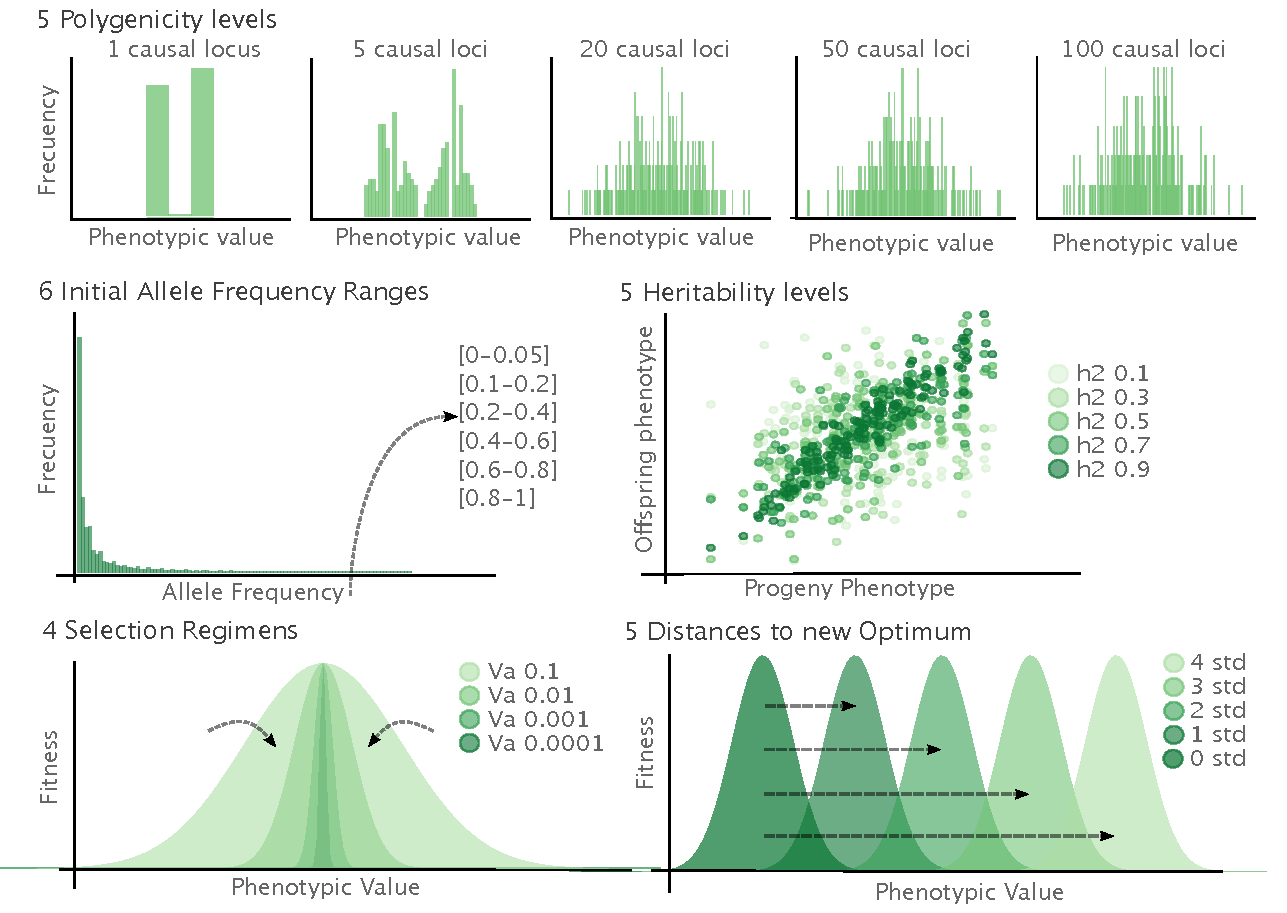
\includegraphics[width=1\textwidth]{figures/parameters.pdf}
  %5\captionsetup{font=small} 
  \caption{Parameters used in the simulations. This figure outlines the comprehensive set of parameters used for the simulations, including the number of contributing loci or polygenicity [1, 5, 20, 50, 100 200], the initial allele frequency ranges of the contributing loci[0-0.05, 0.1-0.2, 0.2-0.4, 0.4-0.6, 0.6-0.8, 0.8-1], the heritability levels [0.1, 0.3, 0.5, 0.7, 0.9], the selection strength modeled as fitness decay [Va=1, 0.1, 0.01, 0.001], and the distance to the new phenotypic optimum modeled as standard deviations from initial phenotypic mean [0, 1, 2, 3, 4, -1, -2, -3, -4]}
  \label{fig:parameters}
\end{figure}

\subsubsection{Population density control}
For all simulations, we set a capacity charge of 900 individuals. The starting population size was 2310 individuals for all simulations, but after the first selection episode, and on every cycle, we randomly subtracted individuals to keep it at 900. This is based on the observations of the real GrENE-net experiment, where the largest populations only reached a maximum of 900 individuals. 

\subsubsection{\textit{A. thaliana} biology}
Because one of our main focuses was to tailor our simulations to the GrENE-net project, we decided to add some characters specific to \textit{Arabidopsis thaliana}, besides the founder populations' genetic diversity. Firstly, we used \textit{A. thaliana}'s mean recombination rate across the genome of $3 \times 10^{-6}$ (cite). Secondly, we simulated non-overlapping generations mimicking the plant annual cycle. Finally, we decided to use strict information about \textit{A. thaliana} reproductive strategies, simulating a 97\% selfing rate, 3\% outcrossing rate (\citep{Platt2010-hy}), and a offspring size taken from $\sim Poisson(7.247)$, based on an experimental average informed from common garden experiments (Exposito-Alonso lab, unpublished). 

\subsubsection{Tree sequence structure to simulate full genomes}
Because we wanted to work with real genetic data to make our simulations highly realistic, we took advantage of the novel tree sequence structure and smooth SliM integration to simulate \textit{A. thaliana} genomes \citep{Kelleher2018-jb, Haller2019-lm}. First, we converted the Variant Call Format (VCF) of the founder population, which included 3,000,000 SNPs, into a tree sequence structure using the Python module Tsinfer \citep{Kelleher2019-ev}. Second, based on each simulation's genetic architecture we selected the loci contributing to the trait value. Thirdly, based on the principle that neutral mutations are merely hitchhikers, we removed them from the tree and saved all mutations not contributing to the trait separately. The resultant tree was lighter and faster to run on SLiM. Lastly, after each simulation concluded, we overlaid the previously removed neutral mutations onto the surviving tree branches, resulting in a comprehensive tree sequence including both neutral and adaptive/non-adaptive mutations.
\url{https://github.com/tskit-dev/pyslim}. 

\subsubsection{Reproducibility}
To ensure the reproducibility and trackability of our analysis, we developed a Snakemake pipeline \citep{Molder2021-ho}. It starts with the initial VCF file from the founder populations and simulates all populations based on the parameter combinations. The pipeline is fully available at \url{https://github.com/Tatianabellagio/slim_grenenet}.

\subsection{Readouts from population simulations}
In addition to obtaining the full genomic dataset at the end of each simulation, we extracted key data at each generation. This included population size, pseudo-environmental variables, individual genetic values, phenotypes, and fitness.

\subsection{Analyses from population simulation readouts}
\subsubsection{Statistical models to explain evolutionary outcomes of populations}
Using the outcomes of the population simulations and their initial parameters, we explored the relationships among these parameters and the populations’ survivorship. We employed Multivariate Linear Regression (MLR) and multiple runs of Logistic Regressions (LR) using the Python module Statsmodels \citep{Seabold2010-ec}. 

\section{Results}
\subsection{Simulation parameters defining population mortality vs adaptation}
To understand how each simulation parameter influences the populations' ability to adapt, we conducted a Multivariate Linear Regression (MLR). We used the parameters as regressors and the populations' survivorship at the 10\textsuperscript{th} generation as the predictor. In Fig. \ref{fig:glm_logisticreg} A, we report the slopes fitted for the MLR divided by the estimated error, i.e., their effect size or t-value for each parameter. This showed that, as expected, the distance to the moving environmental optimum had the strongest impact on the populations' survivorship (estimate = -2.39, t-value = -188.48, $p<1 \times 10^{-30}$), followed by the strength of selection as fitness decay (estimate =-1.95, t-value=-170.88, $p<1 \times 10^{-30}$). Heritability followed, increasing the probability of survival (estimate = 0.65, t-value = 80.144, $p<1 \times 10^{-30}$). Surprisingly polygenicity showed a slight positive effect (estimate =0.25, t-value=32.378, $p=7.77 \times 10^{-3}$) and the frequency of the coding alleles in the initial population showed the smallest impact on the population's survivorship (estimate = -0.04, t-value=-5.33, $p=7.66 \times 10^{-3}$).

Because we expected some of the parameters to have non-linear and context-dependent effects, we then conducted independent logistic regressions for fixed parameter combinations to marginally assess the effect and significance of a given parameter on survivorship (Fig. \ref{fig:glm_logisticreg} B). For this analysis, we obtained a distribution of t-values for each parameter, e.g., polygenicity, against a background of other parameter combinations, e.g., heritability-starting allele frequency-strength of selection-distance to new optimum. We only considered slopes with a p-value lower than 0.05 after Bonferroni correction. This analysis confirmed the MLR results for selection strength and distance to the new optimum, and led us to reevaluate the effects of heritability, initial allele frequency, and polygenicity on population survivorship. These parameters showed a distribution of t-values and estimated coefficients ranging from positive to negative values, indicating diverse impacts on population survivorship.

\begin{figure}[h]
  \centering
  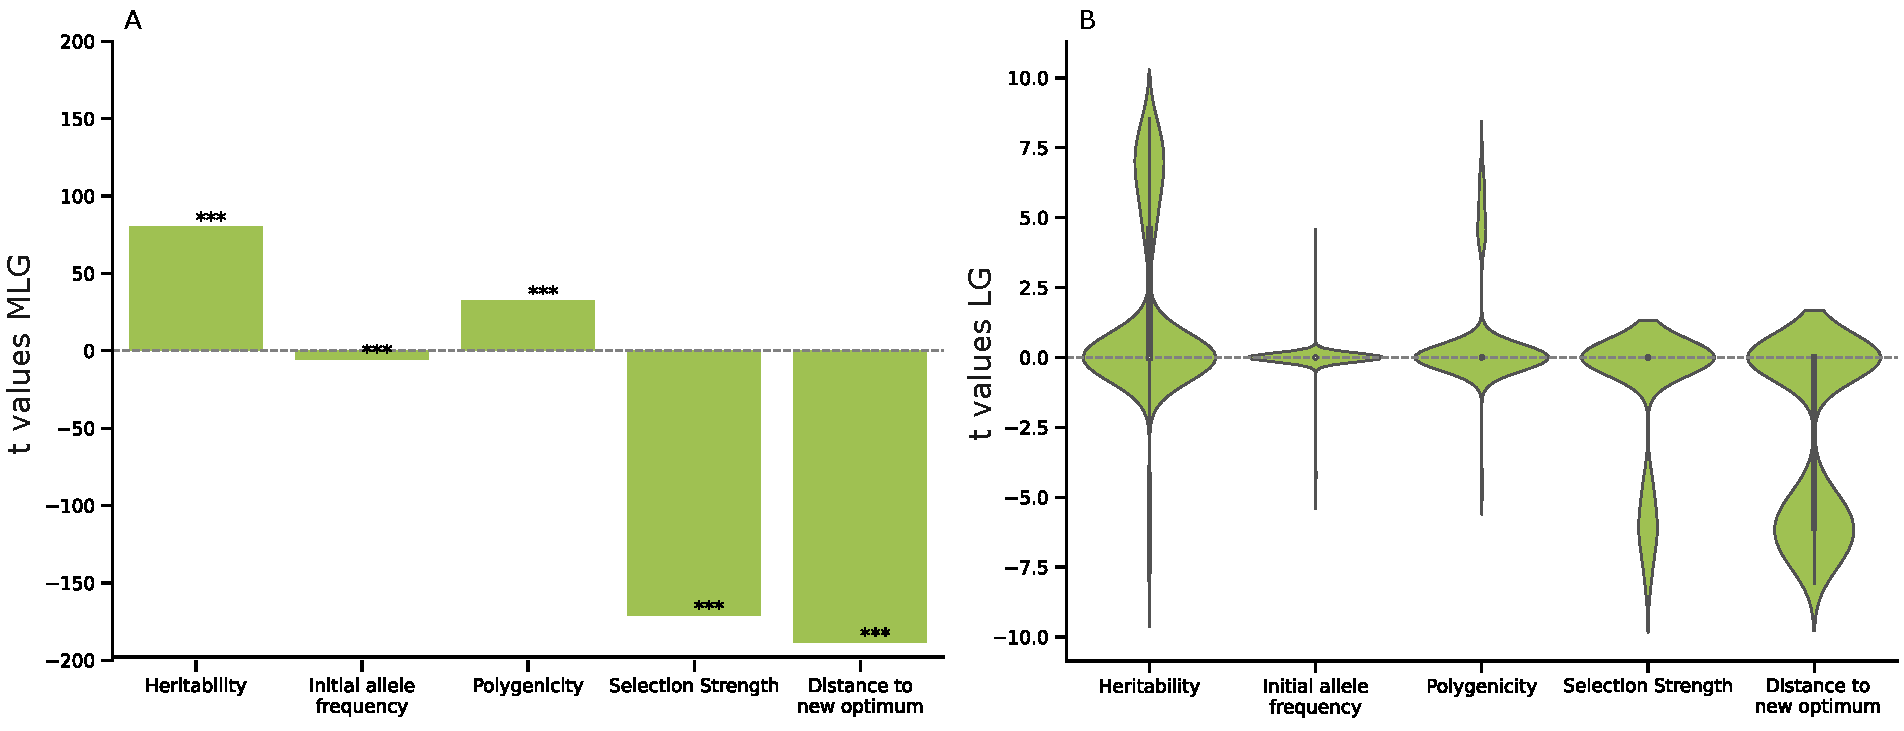
\includegraphics[width=1\textwidth]{figures/glm_logisticreg_newver.pdf}
  \caption{Simulation parameters' impact on populations' survival. Panel \textbf{A} displays the outcomes of the Multivariate Linear Regression (MLR) with all parameters as predictors for binary survival. The bars indicates the MLR t-values. Asterisks denote levels of significance. Panel \textbf{B} shows the results obtained by running the
  Logistic Regressions (LR) for each parameter while holding all others constant. The violin plots represent the distribution of t-values obtained across all LR. Only parameters with p-values less than 0.05 after Bonferroni correction were included.}
  \label{fig:glm_logisticreg}
\end{figure}


\subsection{High polygenic traits enhance a population's adaptability in extreme, novel environments}
When fitness decay is not excessively severe and populations are sufficiently close to the new optimum, polygenicity does not significantly impact a population’s survival probability. This is evident from the t-values near zero (Fig. \ref{fig:poly_panel_figure} A, lower left corner). Nor does it when fitness decay is too steep or the new optimum is very distant, as most populations will inevitably perish regardless of their genetic architecture (Fig. \ref{fig:poly_panel_figure} A, upper right corner).

At the 'extinction edges', defined as the intersection of selection strengths and distance to the new optimum, where populations have a survivorship rate between 10\% and 90\%, we observed a notable pattern (Fig. \ref{fig:poly_panel_figure} A and B, diagonal from upper left to lower right). Here, an increase in polygenicity positively impacts populations' survivorship.(Fig. \ref{fig:poly_panel_figure} C, slope estimate = 0.27, t-value=56.23, $p<1 \times 10^{-30}$). This aligns with population size measurements from Fig. \ref{fig:pop_size_poly_gen10}, where populations with higher polygenic traits are able to conquer environments of new further away optimum, compared with lower polygenic architectures in the 10\textsuperscript{th} generation.

Polygenicity seems to be particularly beneficial in environments with distant optima, under directional selection, but its impact under stabilizing selection is not as pronounced (Fig. \ref{fig:poly_panel_figure}, bottom row). We also observe that polygenicity tends to have a positive effect on survivorship only at higher heritability values (Fig. \ref{fig:poly_panel_figure}). Negative correlations between survivorship and increased polygenicity were observed in only four scenarios, involving very low allele frequencies and distant new optima. (Slope estimates = -7.43, -1.601, -7.19, -0.81, t-values=-4.17 , -4.97, -4.44, -4.52, all $p<1 \times 10^{-5}$). In these cases, we expect that rare phenotypes away from the original optimum but close to the new optimum caused by monogenic architectures may allow a rare advantage.

\begin{figure}[H]
  \centering
  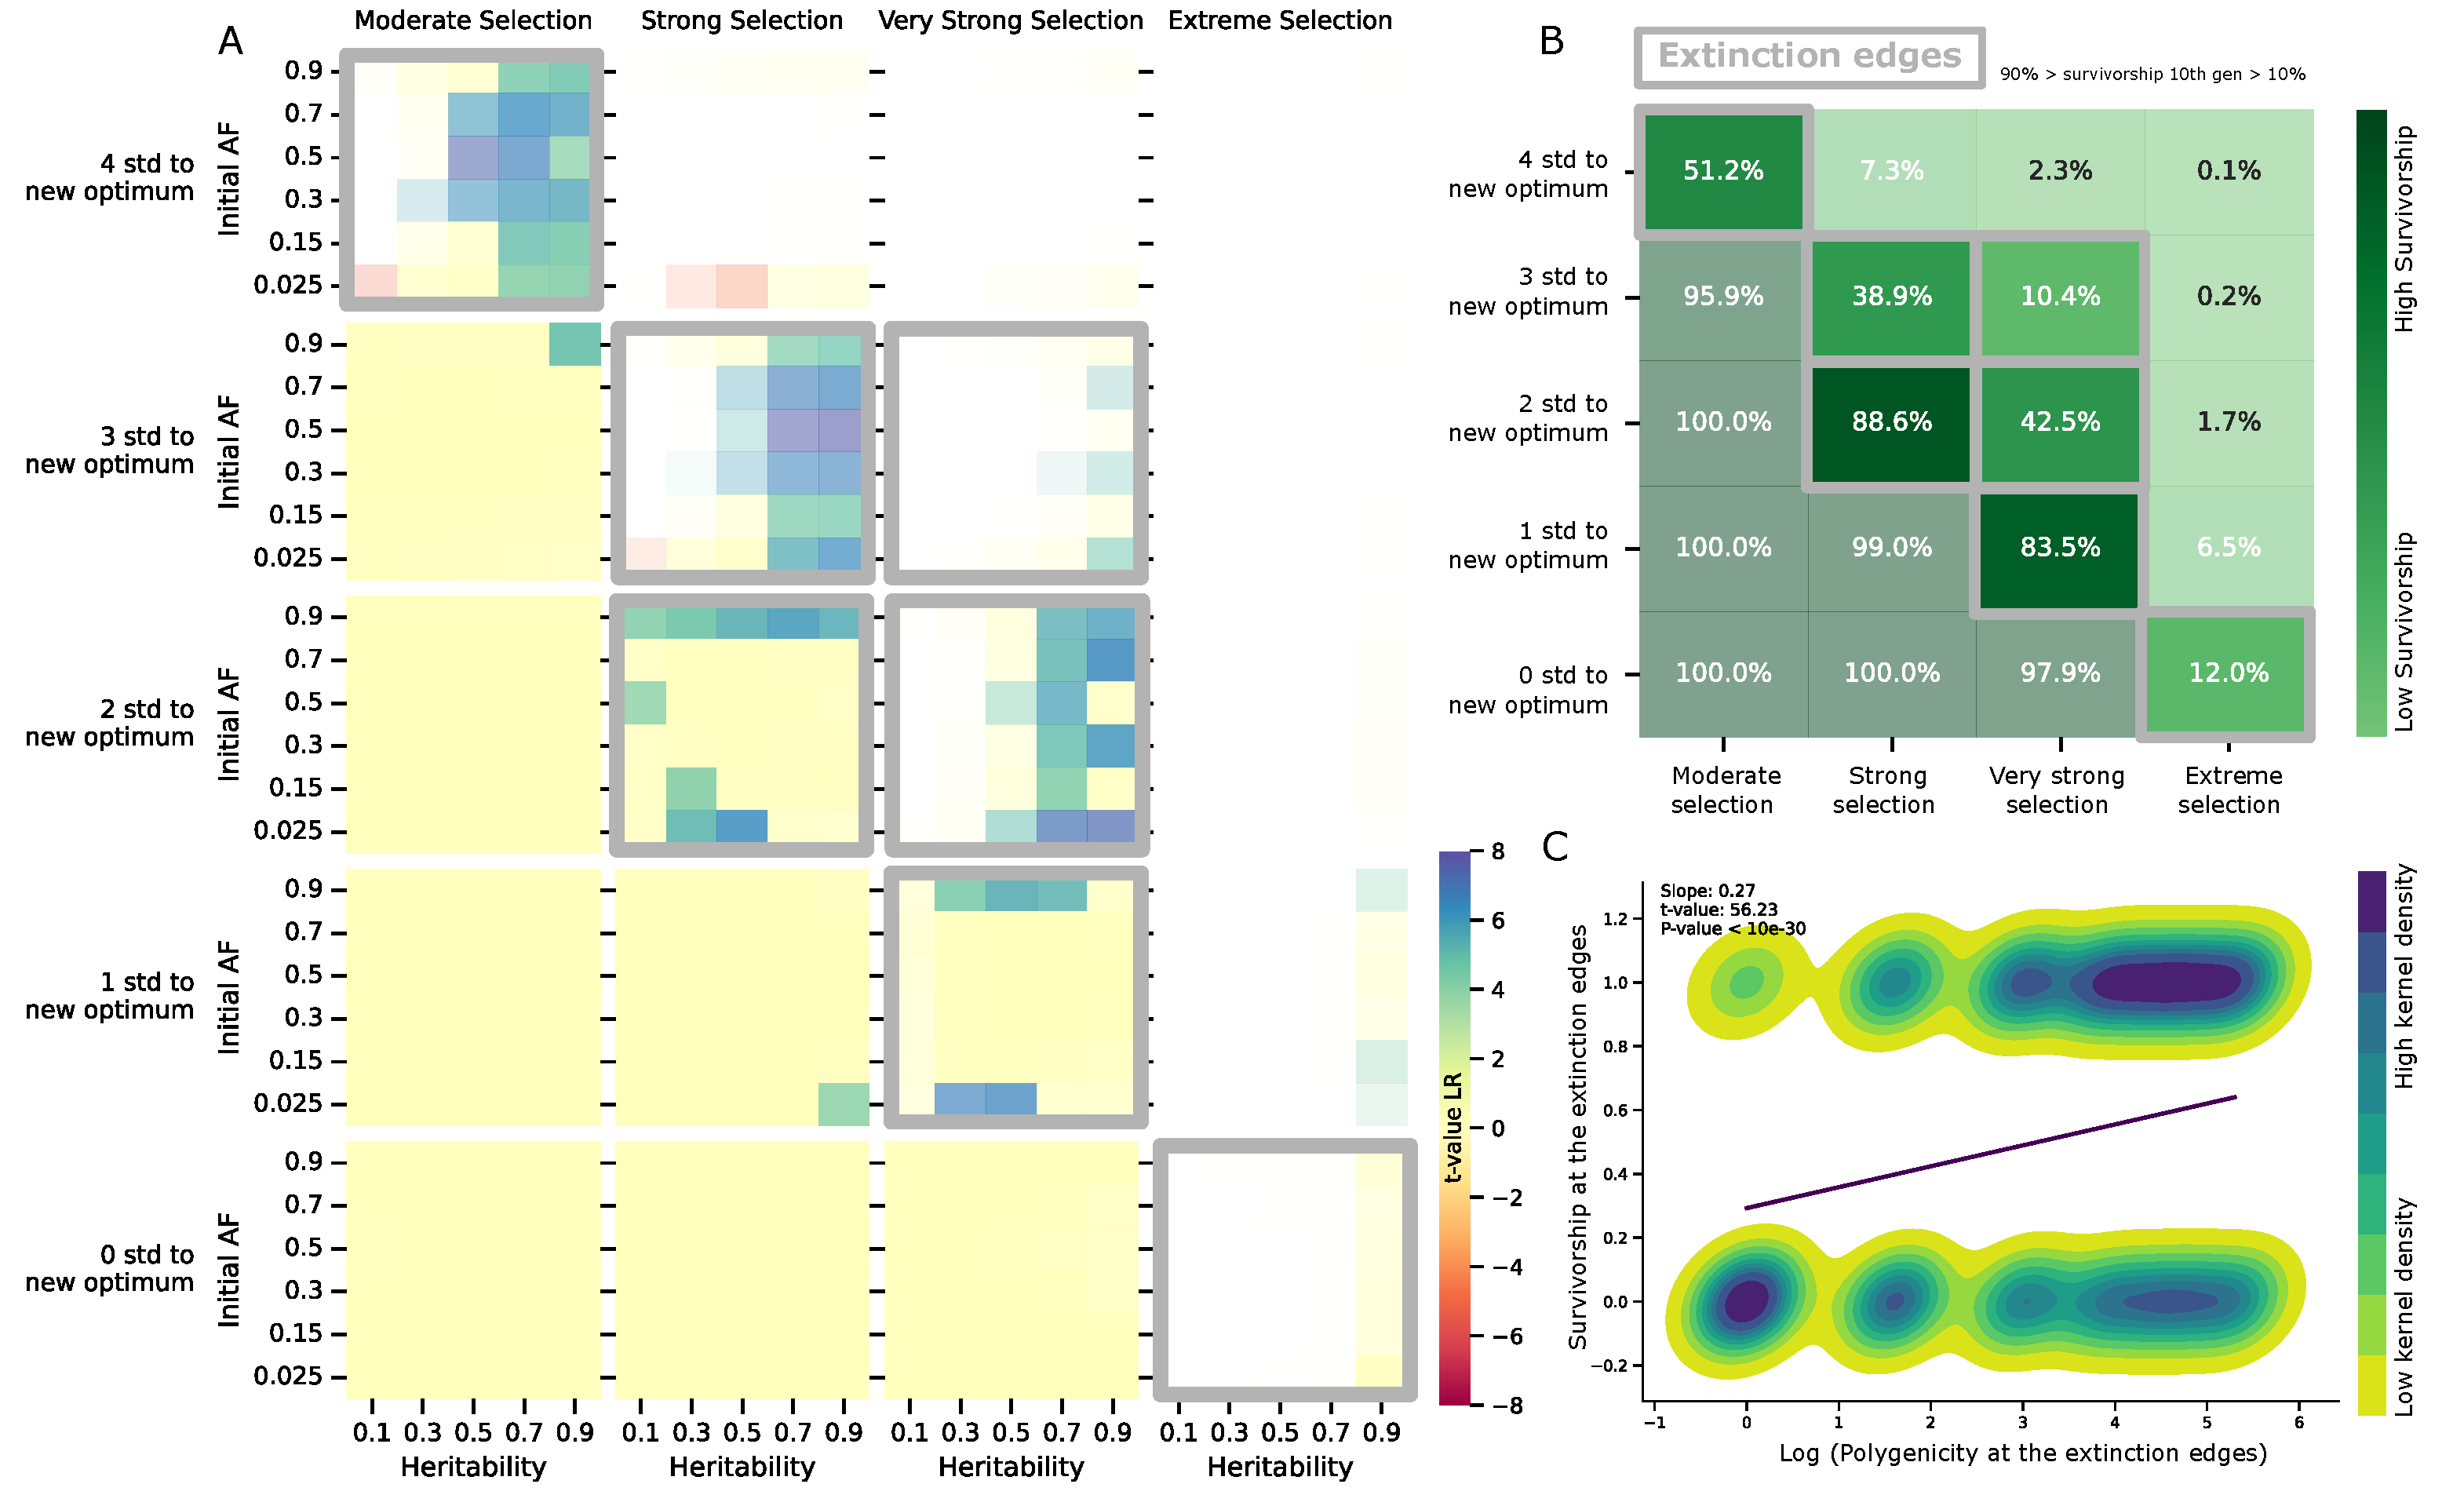
\includegraphics[width=1\textwidth]{figures/poly_survivalship_value_edges.pdf}
  \caption{Impact of polygenicity on populations' survival after the 10\textsuperscript{th} generation. Panel \textbf{A} illustrates the effect of the number of contributing alleles (polygenicity) on populations' survivorship through the fitted logistic regression slopes between polygenicity and survivorship. Each colored square represents one t-value value when all the remaining parameters are kept constant as indicated in the figure's legend (heritability, range of initial allele frequency, distance to new phenotypic optimum and selection strength), providing a comprehensive view of how polygenicity determines adaptation probability in the context of the other parameters. Furthermore, the survival rates of populations are superimposed with varying degrees of transparency, visually emphasizing areas of lower (less transparency) or higher mortality (more transparency). Panel \textbf{B} showcases the 'extinction edges'. When taking into account the two most determining parameters on the population's survivorship -distance to new phenotypic optimum and selection strength- the extinction edges are defined as the combination of these two parameters where the population's survival rates are at least 10\%, but no more than 90\%. In panel \textbf{C}, the positive relationship between survival percentage and an increase in the log of polygenicity at the extinction edges is displayed (slope estimate = 0.27, t-value=56.23, $p<1 \times 10^{-30}$)}
  \label{fig:poly_panel_figure}
\end{figure}

\begin{figure}[H]
  \centering
  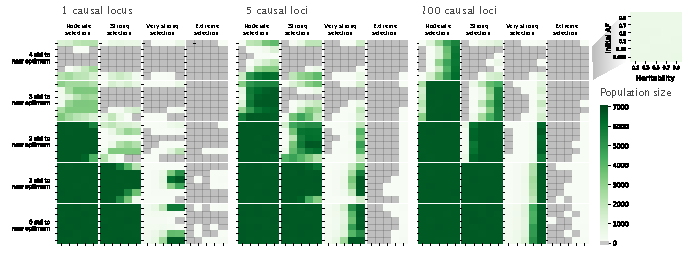
\includegraphics[width=1\textwidth]{figures/pop_size_GEN10.pdf}
  \caption{Populations sizes at generation 10 based on different genetic architectures, selection strength and distance to the new optimum. Each color's square represents the average population size of the simulated replicates based on the given value for initial allele frequency, number of contributing loci, heritability, distance to new optimum, and selection strength at generation 10. When the square is marked in grey, all population replicates under the given conditions went extinct.}
  \label{fig:pop_size_poly_gen10}
\end{figure}

\subsection{High heritability does not consistently enhance a population’s adaptability to new environments}
In concordance with the results of high polygenicity being positive, high heritability is also important to adapt at the extinction edges (Fig. \ref{fig:h2_panel_figure} A). Consistent with the observations in Fig. \ref{fig:glm_logisticreg}, heritability generally has a positive effect on a population's survivorship at the extinction edges (Fig. \ref{fig:h2_panel_figure} B, slope estimate = 2.59, t-value=79.51, $p<1 \times 10^{-30}$). This is also shown in Fig. \ref{fig:pop_size_poly_gen10}, where higher heritability in polygenic architectures consistently conveys the population with a higher population size at further optima.

However, this positive relationship between heritability and survival weakens as the trait's polygenicity decreases (Fig. \ref{fig:h2_panel_figure} B). In scenarios involving traits with polygenic architectures the relationship between heritability and survivorship is the strongest (slope estimate = 1.69, t-value=38.33, $p<1 \times 10^{-30}$), it starts to weaken at low polygenic architectures (slope estimate = 1.05, t-value=19.14, $p<1 \times 10^{-30}$), and it is almost zero for monogenic cases (slope estimate = 0.2, t-value=2.35, $p=1.86 \times 10^{-2}$). Additionally, there are several instances where high heritability leads to lower survival ((Fig. \ref{fig:h2_panel_figure} A red squares). These instances occur under various initial allele frequencies and are specifically observed in low polygenic architectures (slope estimates = -6.13, -7.33, -0.59, -1.81, -1.44, -0.93, -0.76, -0.63, -1.16, t-values=-4.12, -4.39, -4.37, -5.53, -6.26, -6.15, -4.87, -4.61, -5.15, all $p<1 \times 10^{-5}$).

\begin{figure}[h]
  \centering
  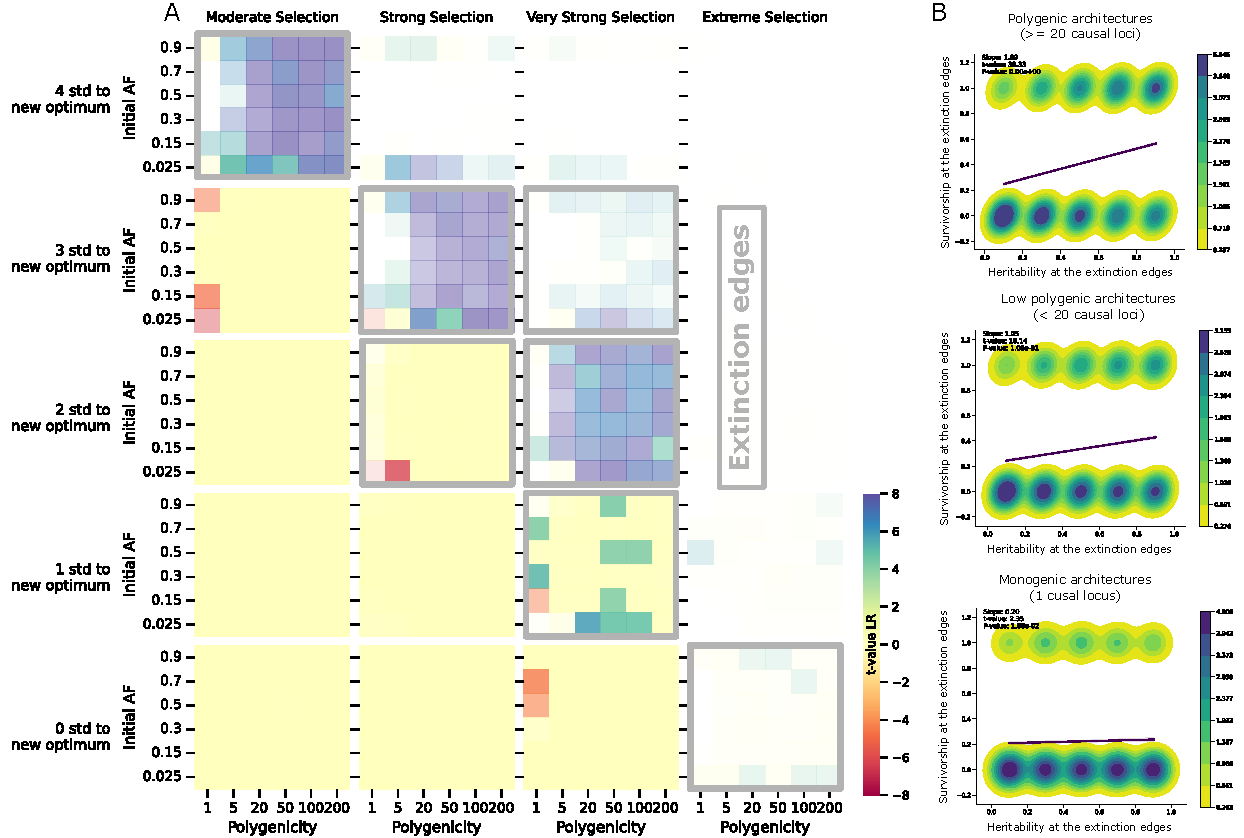
\includegraphics[width=1\textwidth]{figures/heristabilityvs_survivo_edges.pdf}
  \caption{Impact of heritability on populations' survival. Panel \textbf{A} illustrates the effect of heritability on populations' survival rates through the fitted logistic regression t-values between heritability and survivorship. Each colored square represents one t-values when all the remaining parameters are kept constant as indicated in the figure's legend (polygenicity, range of initial allele frequency, distance to new phenotypic optimum and selection strength), providing a comprehensive view of how heritability determines adaptation probability in the context of the other parameters. Furthermore, the survival rates of populations are superimposed with varying degrees of transparency, visually emphasizing areas of lower (less transparency) or higher mortality (more transparency). In panel \textbf{B} the fitted lines for the relationship between the population's survival and heritability at the extinction edges are reported at three different polygenicity levels, showcasing that the relevance of heritability is dependent on the polygenicity level. Polygenic architectures (slope estimate = 1.69, t-value=38.33, $p<1 \times 10^{-30}$), low polygenic architectures (slope estimate = 1.05, t-value=19.14, $p<1 \times 10^{-30}$ ) and monogenic architectures (slope estimate = 0.2, t-value=2.35, $p=1.86 \times 10^{-2}$)}
  \label{fig:h2_panel_figure}
\end{figure}

\subsection{Genetic architecture is a key factor determining mean fitness and fitness variance at the extinction edges}
Based on the context-dependent results of the connection between genetic architectures and population survival, we further explored the evolutionary dynamics based on genetic architecture at the extinction edges. We zoomed into the simulations with selection strength of $Vs=0.01$ and where the new optimum is 2 standard deviations from the original population phenotypic mean, as this is the parameter space that led to significant and varying correlations of genetic architecture with population's survival (Fig. \ref{fig:pop_size_poly_gen10}, Fig. \ref{fig:poly_panel_figure}). 

In simulations with high heritability levels (Heritability = 0.9), we observed that populations with more polygenic architectures achieved higher mean fitness ($\bar{w}$) and fitness variances ($V_w$)compared to those with lower polygenic traits (Fig. \ref{fig:mean_fitness_acrossgen}, Fig. \ref{fig:var_fitness_across_gen}). Specifically, the mean of $V_w$ across all initial allele frequencies at the 10\textsuperscript{th} generation was $0.02$ for 1 causal locus, $0.08$ for 5 causal loci, and $0.09$ for $\geq 20$ causal loci. Correspondingly, the mean $\bar{w}$ across all initial allele frequencies at the 10\textsuperscript{th} generation was $0.1$ for 1 causal locus, $0.47$ for 5 causal loci, and between $0.64- 0.65$ for $\geq 20$ causal loci. Notably, the variance in $\bar{w}$ and $V_w$, across initial allele frequencies and their replicates exhibits a striking contrast when comparing low and high polygenic architectures at high heritability levels in the final generation. For instance, the variance in $V_w$ was $1.445 \times 10^{-3}$ for 1 causal locus, $1.149 \times 10^{-3}$ for 5 causal loci, and between $1.7-4.1 \times 10^{-5}$ for $\geq 20$ causal loci, while the variance of $\bar{w}$ was $3.6 \times 10^{-2}$ for 1 causal locus, $5.8 \times 10^{-2}$ for 5 causal loci, and between $3 \times 10^{-3} - 2.8 \times 10^{-4}$ for $\geq 20$ causal loci. This pattern underscores the fact that low polygenic architectures lead to more stochastic simulation outcomes, where the idiosyncrasy created by only one or few alleles controlling the trait leads to more variable $\bar{w}$ and $V_w$ across population simulations. Oppositely, high polygenic architectures have $\bar{w}$ and $V_w$ that are more consistent across population simulations and are less affected by the randomness of the initial conditions.

Intriguingly, low heritability (Heritability = 0.1), resulted in more robust starting $\bar{w}$ and $V_w$, than high heritability cases (Fig. \ref{fig:mean_fitness_acrossgen}, Fig. \ref{fig:var_fitness_across_gen}). The mean $V_w$ across all initial allele frequencies at the 10\textsuperscript{th} generation was $0.035$ for 1 causal locus, $0.066$ for 5 causal loci, and between $0.066-0.082$ for $\geq 20$ causal loci, while the mean $\bar{w}$ across all initial allele frequencies at the 10\textsuperscript{th} generation was $0.069$ for 1 causal locus, $0.136$ for 5 causal loci, and between $0.14-0.15$ for $\geq 20$ causal loci. We believe these results explain the observations in Fig. \ref{fig:h2_panel_figure}, where low heritability correlated positively with survival in low polygenic architectures. 

\begin{figure}[H]
  \centering
  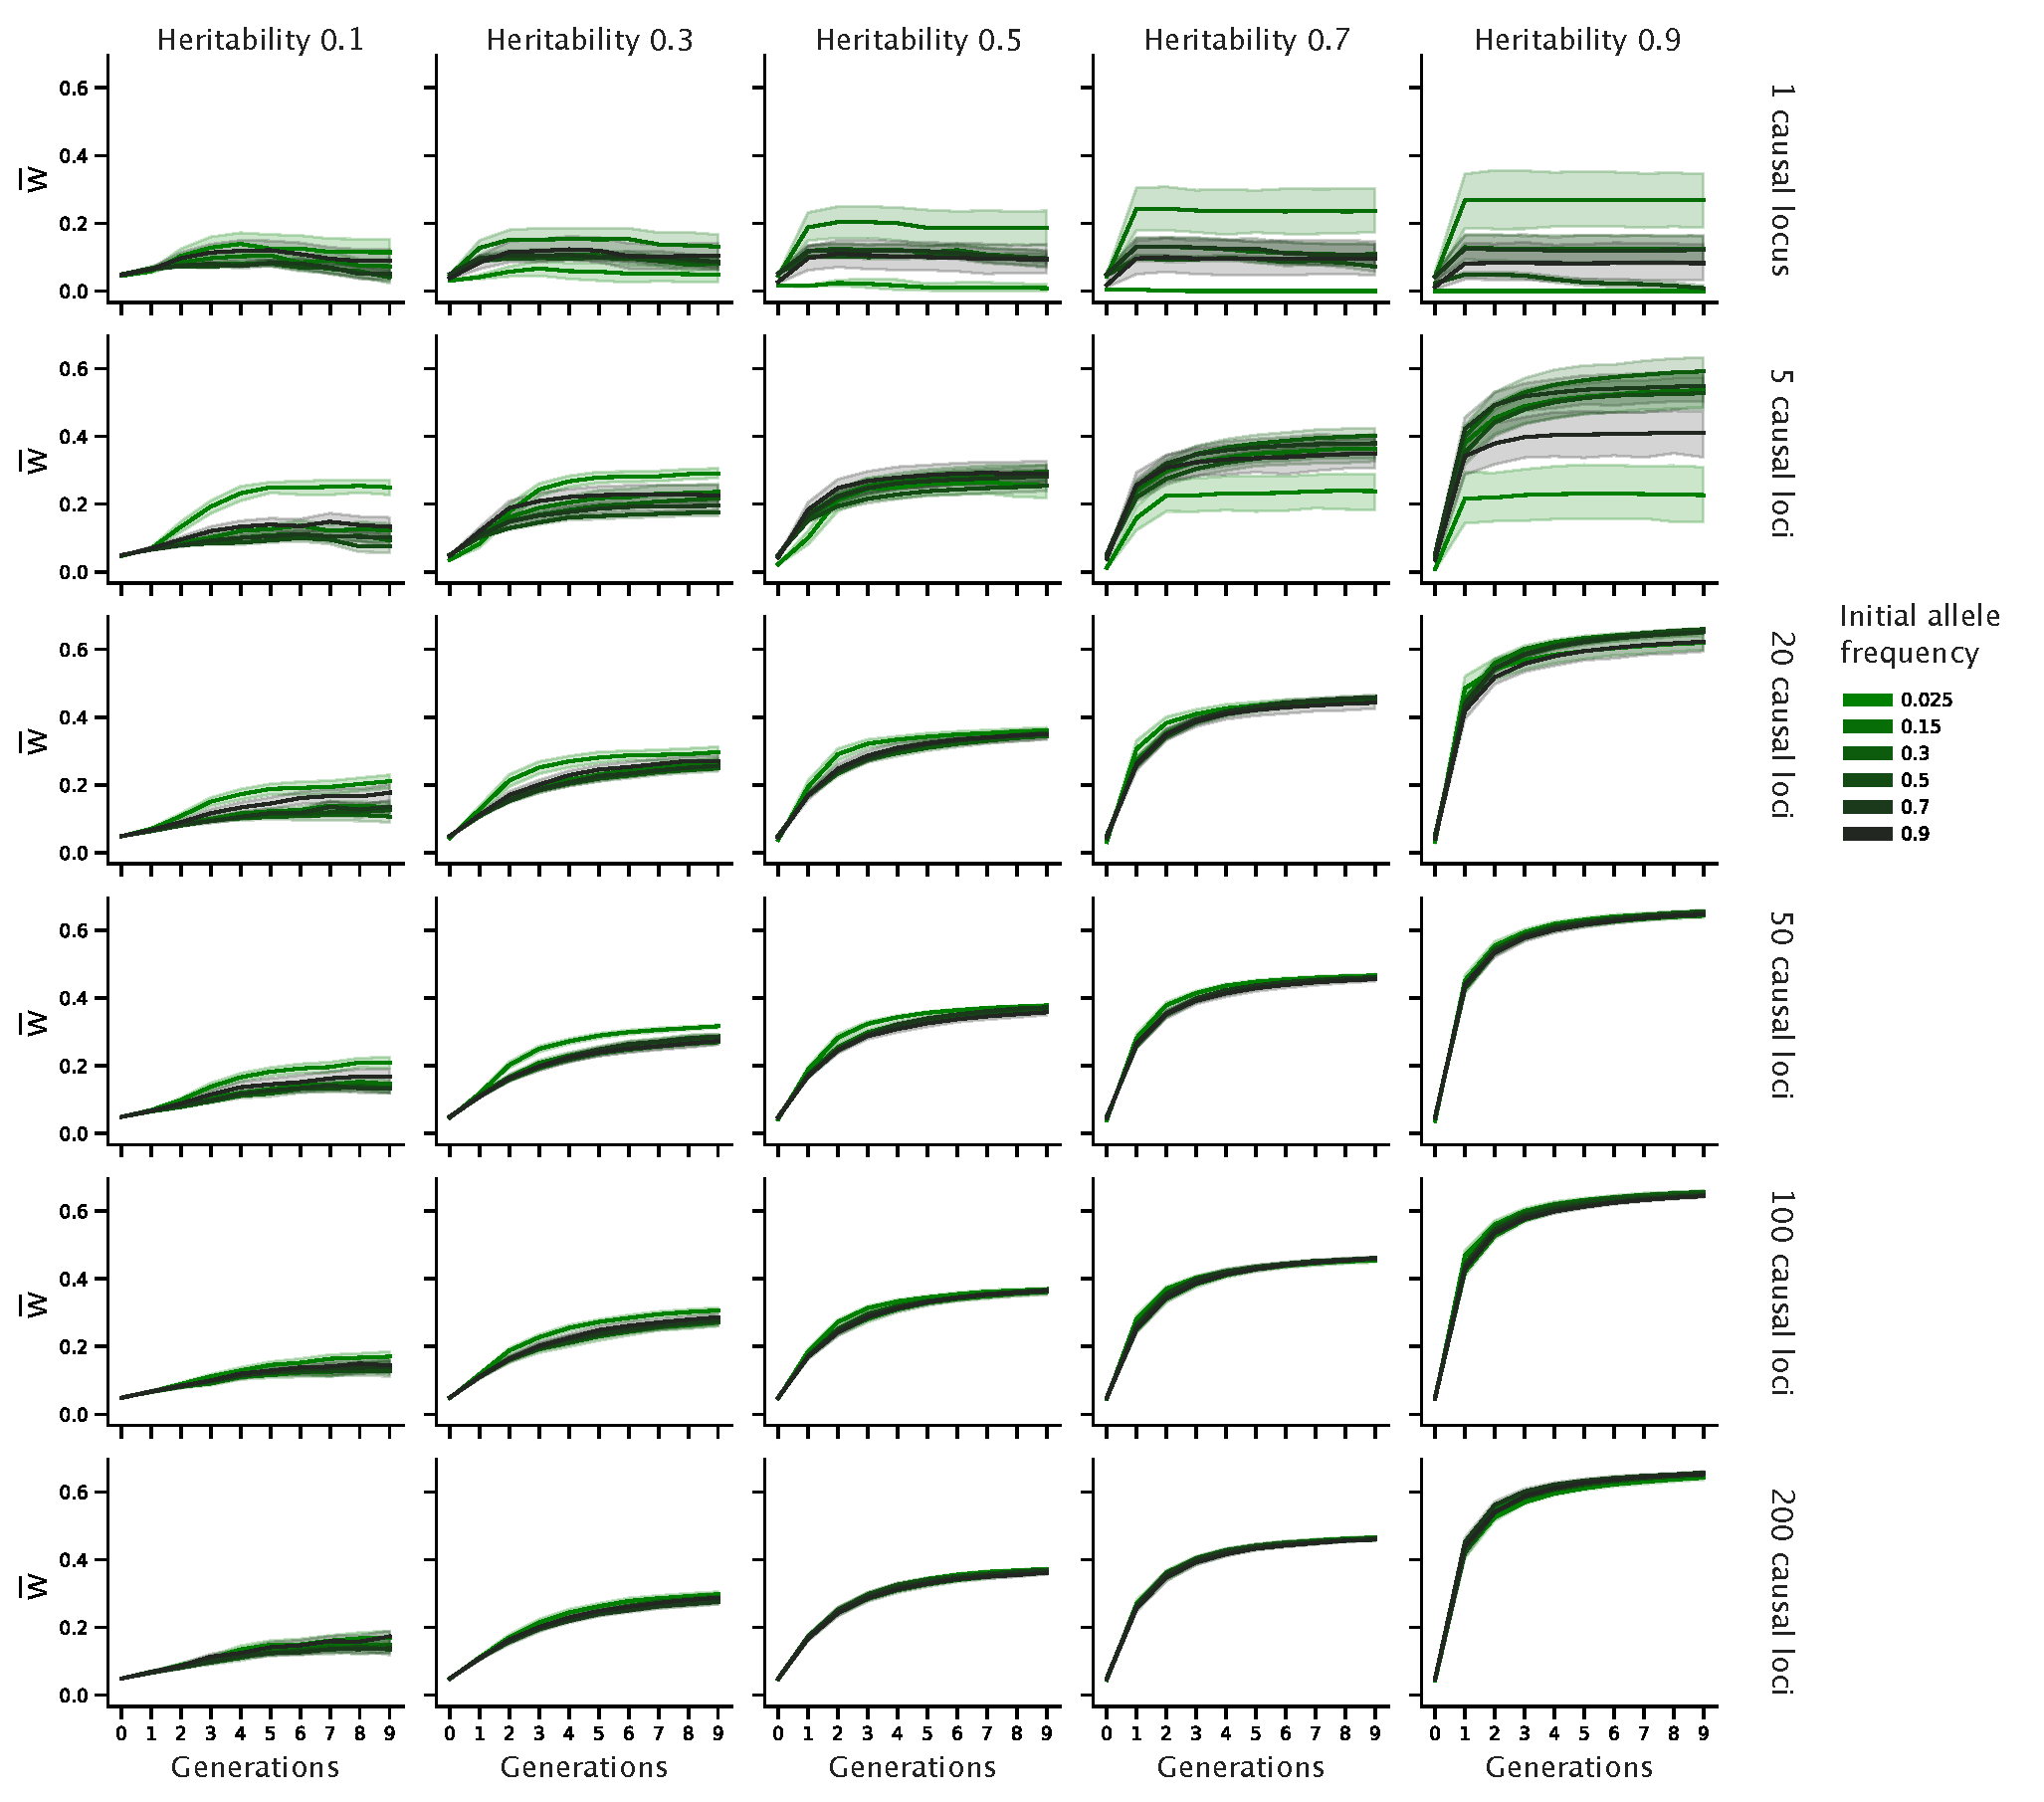
\includegraphics[width=1\textwidth]{figures/mean_fitness_acrossgen.pdf}
  \caption{Evolution of $\bar{w}$ at the extinction edges based on genetic architecture. Changes in $\bar{w}$ across generation for different initial allele frequencies, polygenicity, and heritability levels. These results correspond to simulations with a fixed selection strength of Vs = 0.01 and whose new optimum was situated 2 standard deviations from the initial population phenotypic mean.}
  \label{fig:mean_fitness_acrossgen}
\end{figure}

\begin{figure}[H]
  \centering
  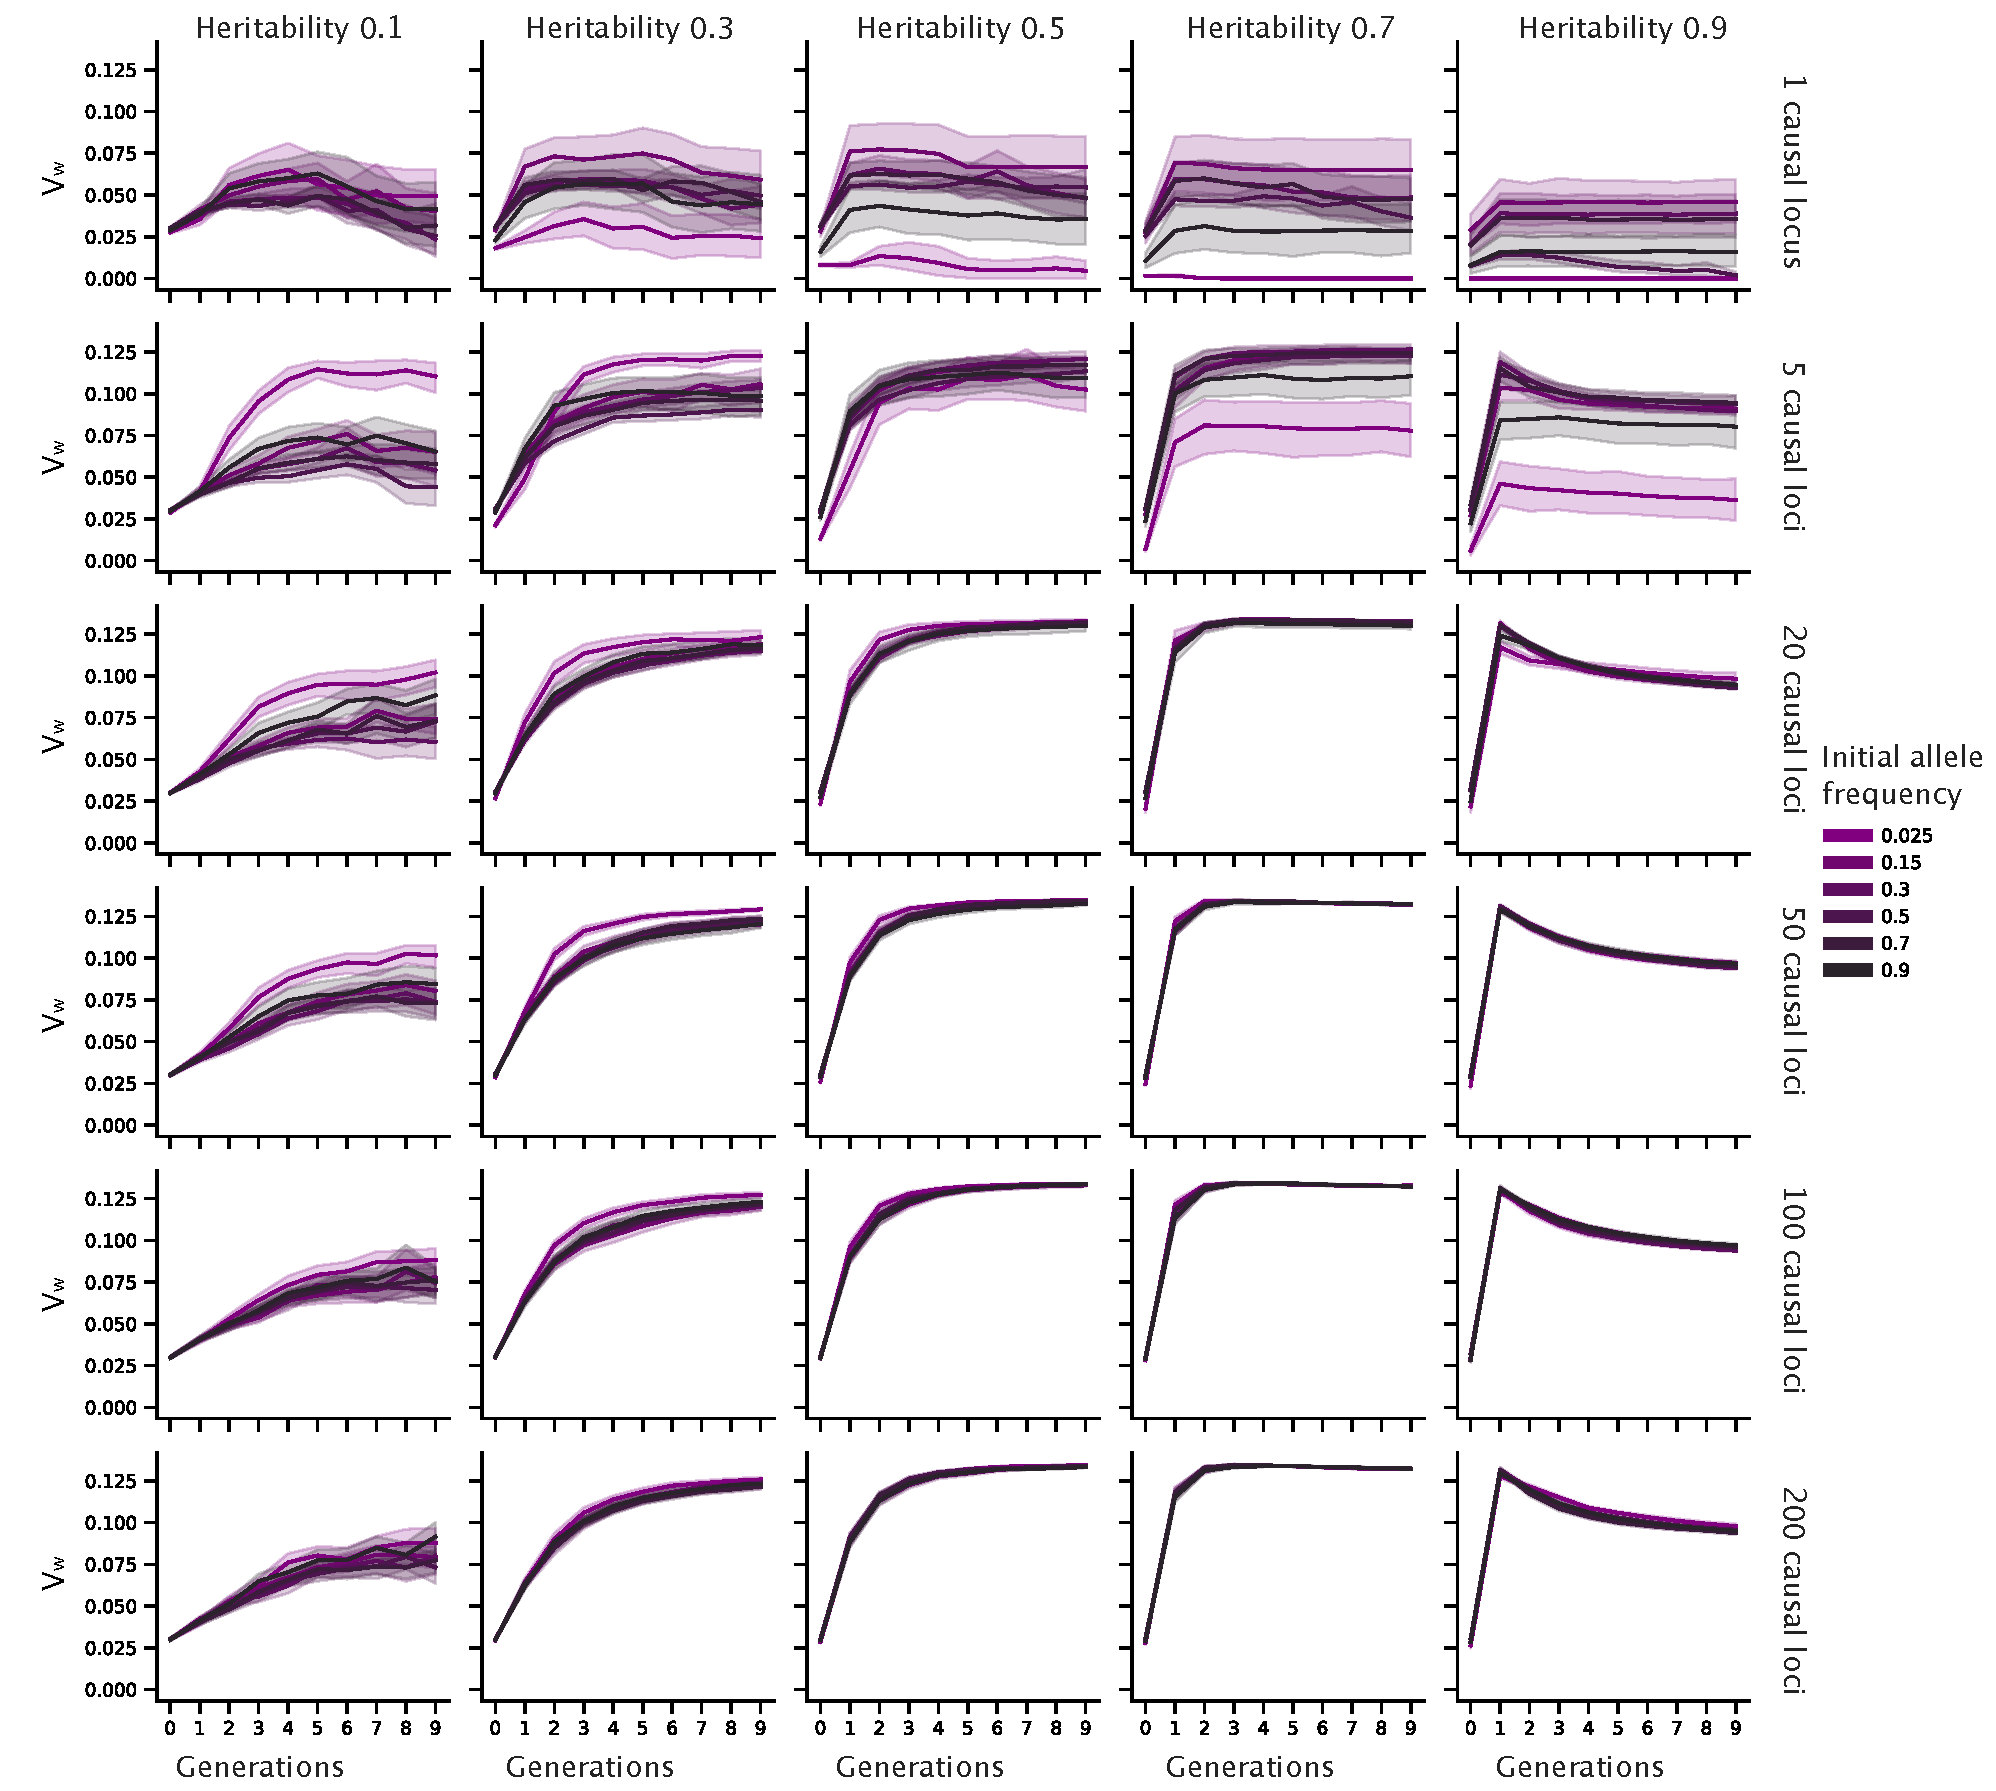
\includegraphics[width=1\textwidth]{figures/var_fitness_across_gen.pdf}
  \caption{Evolution of $V_w$ at the extinction edges based on genetic architecture. Changes in $V_w$ across generation for different initial allele frequencies, polygenicity and heritability levels. These results correspond to simulations with a fixed selection strength of Vs = 0.01 and whose new optimum was situated 2 standard deviations from the initial population phenotypic mean.}
  \label{fig:var_fitness_across_gen}
\end{figure}

\section{Discussion}
\subsection{Understanding rapid evolution in a changing world}
With environments changing faster than ever, understanding the evolutionary dynamics of rapid adaptation has become of utmost interest. Application of this knowledge ranges from invasive species management \citep{Lee2002-jg, Lee2008-cd}, applied evolutionary rescue for species at extinction risk, or even understanding concerning medical issues such as the emergence of novel infectious diseases where genetic adaptation to a novel host is required \citep{Holt2002-fn, Antia2003-in}.

Rapid adaptation has been widely documented as shown in the examples listed in the introduction. Nonetheless, this does not mean that it can always occur. The mentioned examples highlight the potential, in principle, for rapid adaptation to overcome environmental changes. However, the large declines of populations across species could be indicative that adaptation to rapid environmental changes is not the rule \citep{ias_ipbes_2023}. Decades ago, theoretical work with simplified population genetic models concluded that regardless of the genetic model, even populations with the necessary genetic variation to adapt, may still often fail to do so in novel environments \citep{Gomulkiewicz1995-sj}. We therefore need to better understand when evolutionary outcomes will fail, and for that, we need a better understanding on key evolutionary and population parameters in realistic simulations and experiments. For example, it is now widely regarded that the probability of a population survival increases with both population size and the number of exchangeable loci (diversity) \citep{Newman1997-tx, Markert2010-wc, Nabutanyi2022-jb}. By identifying measurable parameters describing the genetics of a species, we may be able to improve practical management decisions for species conservation. 

\subsection{Genetic architecture implication on population's fitness}
In our realistic simulations, we showed that increased trait polygenicity had a positive effect on populations' survivorship probability at the extinction edges (Fig. \ref{fig:poly_panel_figure}) and enabled populations to adapt to environments further from their original optimum (Fig. \ref{fig:pop_size_poly_gen10}). Additionally, our results revealed that these populations consistently exhibited higher  $\bar{w}$ and $V_w$ after the short period of 10 generations (Fig. \ref{fig:mean_fitness_acrossgen}, Fig. \ref{fig:var_fitness_across_gen}). 

Previous literature on the relationship between rapid evolutionary outcomes and genetic architecture has been inconclusive. Gomulkiewicz \& Holt’s foundational work examined both a quantitative-genetic model and a one-locus model, finding similar evolutionary outcomes. \citep{Gomulkiewicz1995-sj}. Orr and Unckless later highlighted evidence favoring polygenic architectures, arguing that it would be difficult for a single locus to adapt to rapid environmental changes compared to multiple loci, a concept now referred to as genetic redundancy \citep{Laruson2020-kd}. However, in later theoretical work, Gomulkiewicz analytically showed that increasing the number of loci contributing to a trait can slow down adaptation, potentially preventing evolutionary rescue \citep{Gomulkiewicz2010-wr}.

Our study's results differ from those of Gomulkiewicz et al., primarily due to the fundamental differences in the underlying assumptions of each study. They use an additive Malthusian fitness model where the population's average fitness at any time is the sum of each contributing locus's fitness. Additionally, they assume constant initial $\bar{w}$ across architectures, leading to a reduced impact of each locus on the overall fitness as the number of loci increases. Based on this, the dilution of the selection coefficients at each locus makes higher polygenic architectures less adaptive than low polygenic ones. The reverse assumption, where Malthusiam fitness is not scaled by the number of loci, would clearly show the opposite. When instead of assuming $\bar{w}$ is constant, but rather selection per locus is constant, is easy to show that fitness would grow linearly with the number of adaptive loci. This assumption would also be problematic. In contrast, the model underlying our realistic simulations does not assume initial constant $\bar{w}$ nor $V_w$ across architectures, instead, we scaled the adaptive trait of our population to have the same mean and variance across architectures. This assumption is achieved by standardizing all phenotypes ($z$) to mean 0 and variance 1. Consequently, we assume that higher polygenic traits will have smaller per locus $V_a(z)$, by also diluting the total $V_a(z)$ into the number of contributing loci. Nevertheless, as shown in Fig. \ref{fig:initial_pop_meanandvar_fitvar} A, when heritability is high, we observe the initial $\bar{w}$ and $V_w$ is highly dependent on the genetic architecture. It can be already noticed that high polygenic architectures have overall higher $\bar{w}$ values at simulation onset, despite the underlying phenotype distributions across architectures being equal. 

\subsection{Genetic architecture and Fisher's fundamental theorem of adaptation}
Fisher's fundamental theorem of adaptation, states that the additive genetic variance in fitness ($V_w$) determines the rate of adaptation over generations (Fisher, 1930). The fact that, at simulation onset, the mean $V_w$ across high polygenic architectures is higher than across low polygenic ones (Fig. \ref{fig:initial_pop_meanandvar_fitvar}) could be enough to explain our results. Again, this supports the notion that the distribution of $V_w$ is highly dependent on the genetic architecture despite starting phenotype frequencies remaining the same, a pattern not accounted for in previous theoretical and simulation work \citep{De_Vladar2014-xp, Orr2014-yn, Stephan2016-tx, Jain2017-mb, Stetter2018-st, Hollinger2019-lb,Thornton2019-ww, John2020-xc}. Furthermore, previous studies have not explored the joint important parameter of varying heritability levels and finite population sizes or other realistic population parameters. The explanation for why low polygenic architectures, already at the simulation onset, show lower mean $V_w$ and an increase in the $V_w$ variance requires further investigation. Our initial hypothesis is related to the nature of low polygenic traits, where the number of possible phenotypes is scarcer and highly dependent on the initial allele frequency of the contributing loci. This is supported by the fact that low polygenic architectures do not always have lower initial $V_w$, but the phenotypic outcome is heavily influenced by initial allele frequencies, leading to stochastic distributions and highly variable $V_w$ (Fig. \ref{fig:initial_pop_meanandvar_fitvar}, Fig. \ref{fig:mean_fitness_acrossgen}, Fig. \ref{fig:var_fitness_across_gen}).

Additionally, our findings align with the more recent studies by Kardos \& Luikart \citep{Kardos2021-jd}. In their study, they used simulations to develop more realistic scenarios relevant to conservation biology, and demonstrated that population extinction is less likely in models with polygenic architectures compared to models with few large-effect loci. The authors interpret that this is due to low-polygenic traits having lower short-term evolutionary potential, although an underlying statistical or mathematical mechanism was not provided.

\begin{figure}[H]
  \centering
  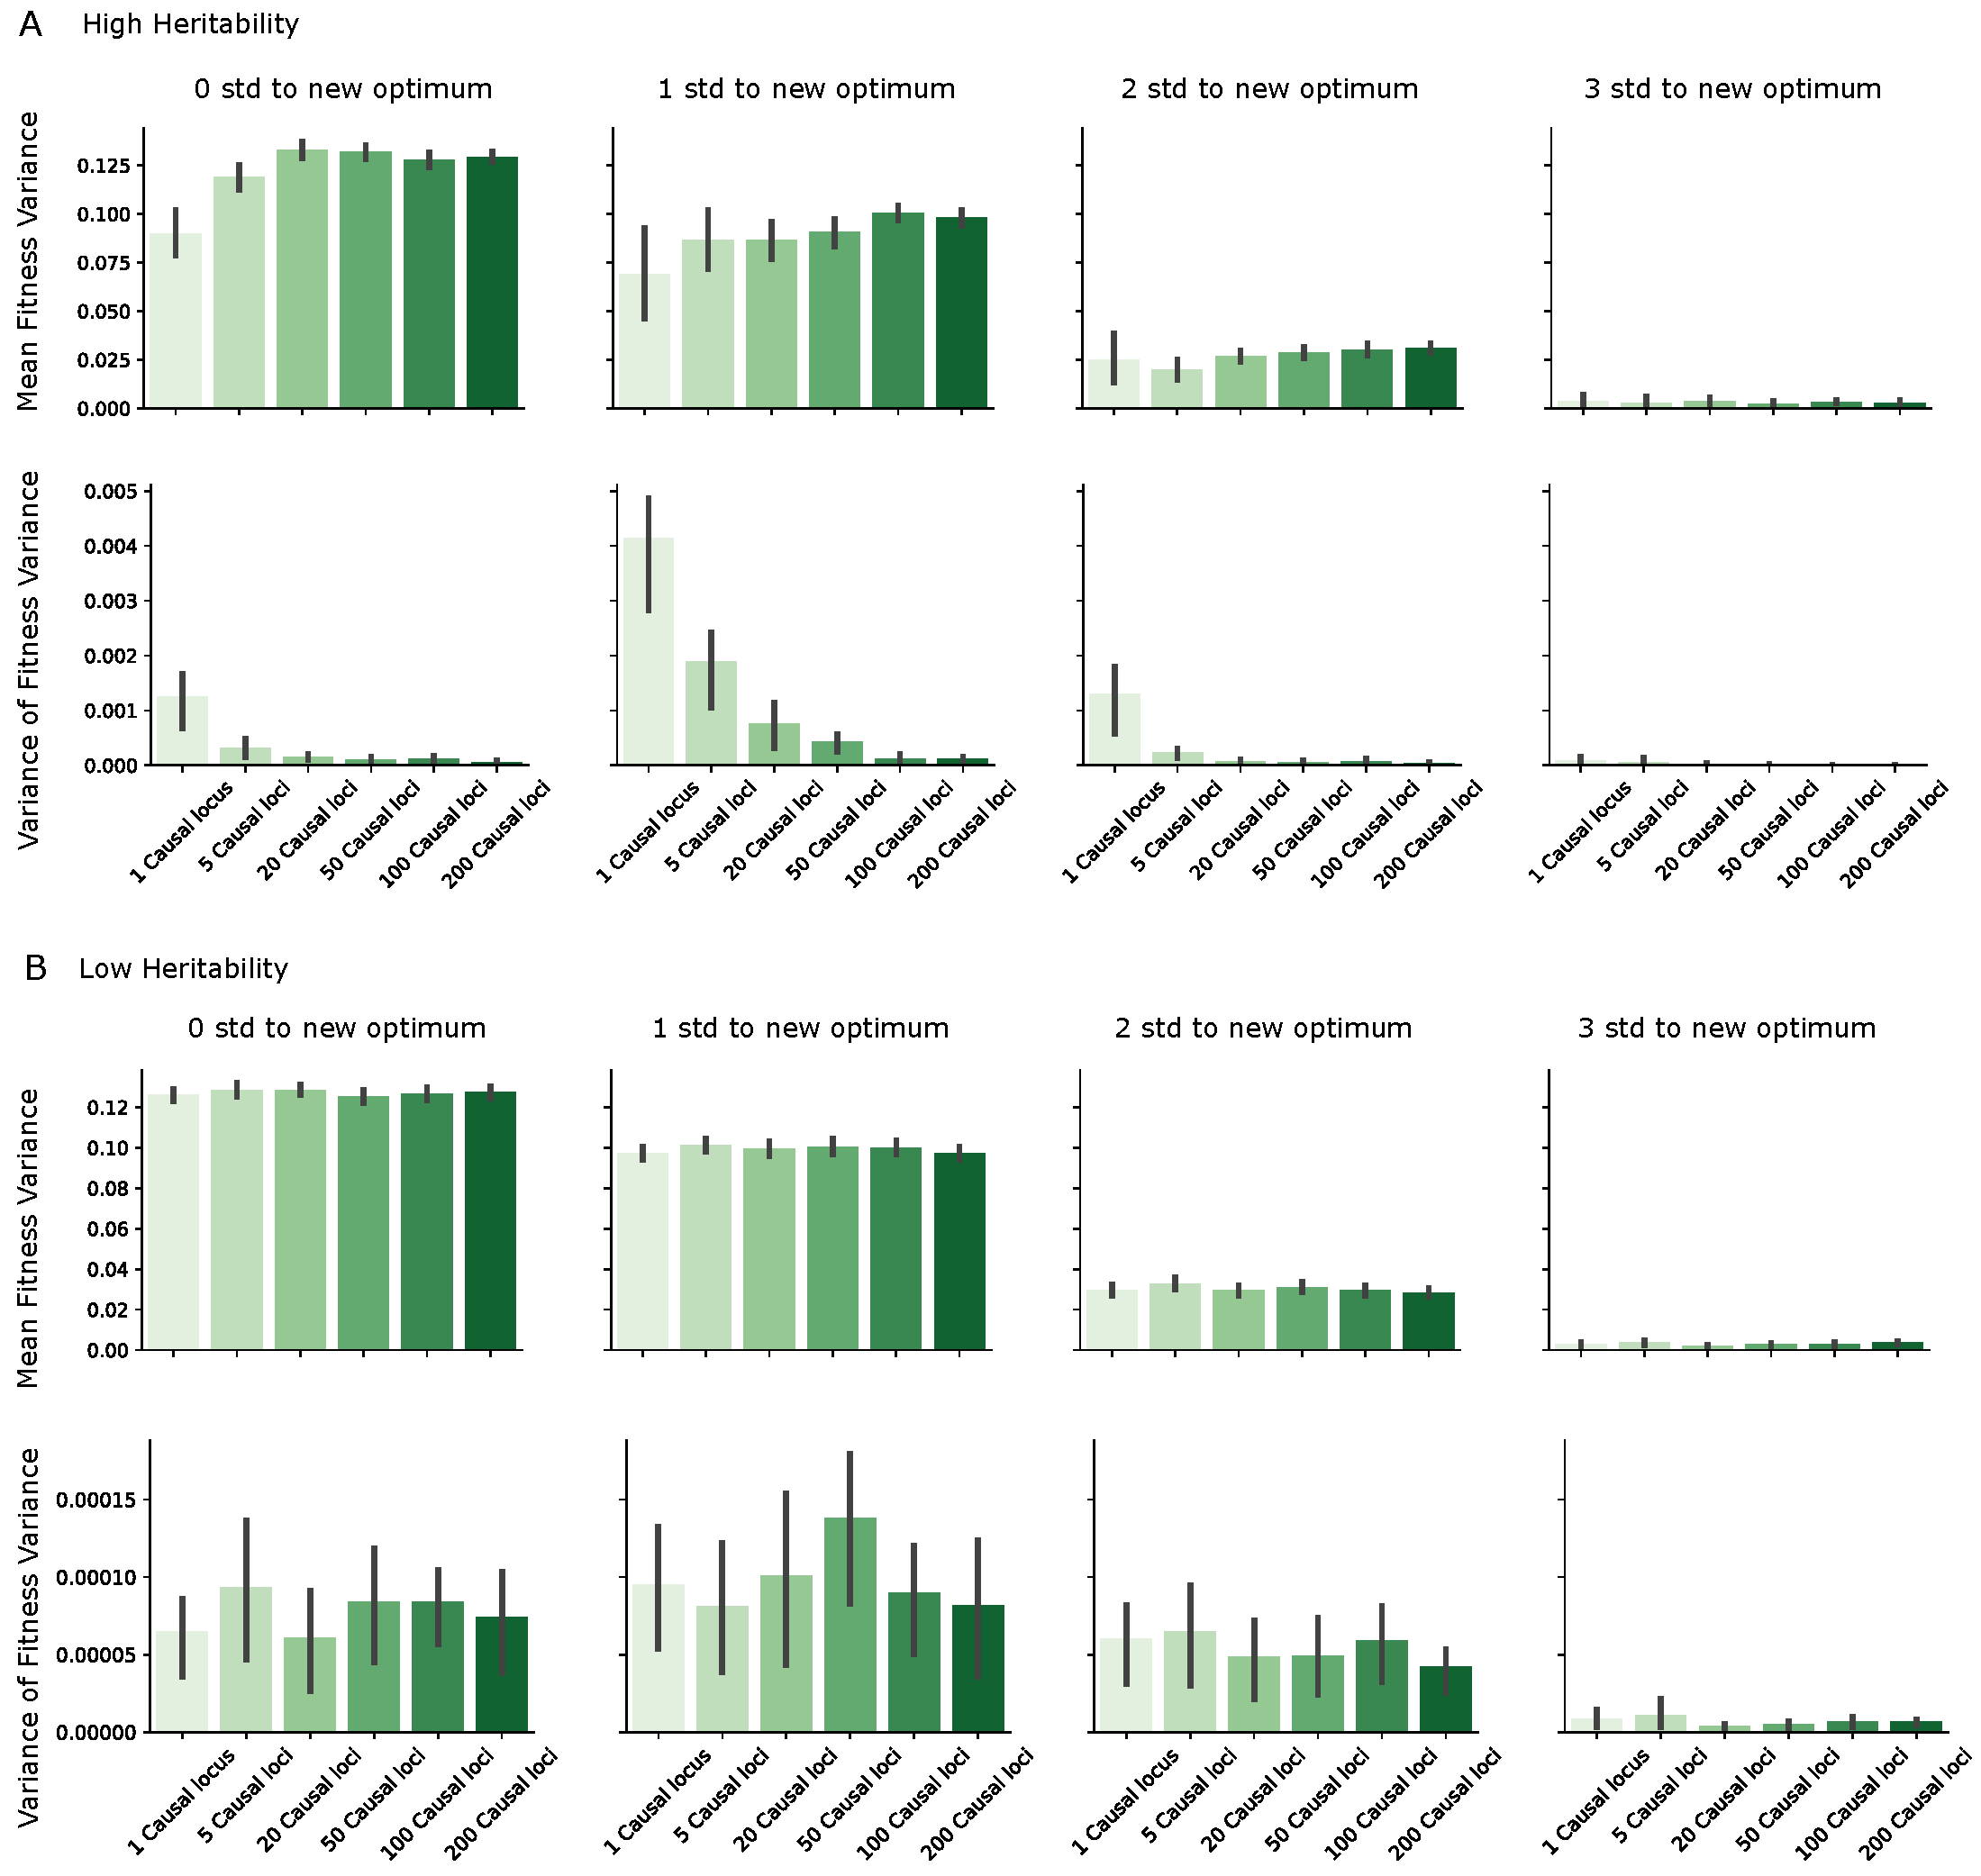
\includegraphics[width=1\textwidth]{figures/mean_var_of_fitness_var_ipop_sel0.1.pdf}
  \caption{Mean $V_w$ and $V_w$ variance of initial populations across genetic architectures and distance to new optimum values at high and low heritability levels and strong selection. The mean $V_w$ and the variance of the $V_w$ for each level of polygenicity were calculated across all initial allele frequencies for the contributing loci and a regimen of strong selection (Vs = 0.1). Panel A displays simulations with a high heritability level of 0.9 and panel B displays simulations with a low heritability level of 0.1}
  \label{fig:initial_pop_meanandvar_fitvar}
\end{figure}

\subsection{The paradox of heritability in low complexity traits}
Contrary to intuition, our results showed that high heritability does not necessarily enhance survival in low-complexity genetic architectures in certain extreme environments. Even more strikingly, in some cases, we found a negative relationship between increased heritability and population survival (Fig. \ref{fig:h2_panel_figure}). Interestingly, the pattern described in the section above is completely masked in initial populations with low heritability levels. At simulation onset, low and high polygenic architectures show similar values of mean $V_w$, and low polygenic architectures do not show higher variance of $V_w$ either (Fig. \ref{fig:initial_pop_meanandvar_fitvar} B). Low heritability seems to introduce a 'buffering' effect, smoothing the phenotypic distribution and consequently fitness, while high heritability and low polygenicity led to strongly discrete phenotypes. 

Finally, we would like to highlight that, because our simulations were designed to be highly realistic and to match a real-world evolutionary experiment (GrENE-net) with \textit{Arabidopsis thaliana}, there could be concerns that our results are influenced by specific genetic characteristics of this species. This would include, high-linkage levels and a notable lack of homozygosity in the populations, which are indicative of alleles not being in Hardy-Weinberg equilibrium. Therefore, we conducted a set of additional simulations under the Wright-Fisher model (i.e. without any realistic and \textit{Arabidopsis thaliana} specifications). These simpler, organism-agnostic simulations (not shown) supported these findings. Furthermore, our conclusions are drawn in the context of rapid adaptation solely based on standing variation. In scenarios where standing genetic variation alone is insufficient to reach the new trait optimum, and \textit{de novo} becomes necessary, our observations might not hold. 

\section{Conclusion}
We conclude that, if the population possesses the genetic diversity to adapt to the newly imposed environmental optimum, polygenic architectures show lower extinction rates and are better suited to adapt and survive in environments with further values from the original optimum due to their higher and more consistent overall mean $V_w$. Furthermore, while heritability is highly beneficial at high polygenic architectures, we had the counterintuitive finding that certain extreme environments and low polygenic architectures would have a lower probability of survival with highly heritable traits. We conclude low polygenic architectures show higher extinction rates across simulation replicates, as their fitness distribution is highly dependent on the initial allele frequency of contributing loci making them generally more susceptible to an extinction event. 

\bibliography{paperpile,extra}

\end{document}
